\section{Experiments}

\subsection{Design}
In order to offer the best possible service, we need to properly tune every factor on which the system depends on:
\begin{itemize}
    \item cashier service rate $\mu_C$
    \item kitchen service rate $\mu_K$
    \item odds of an order being a Simple one $\pi_S$= 1-$\pi_C$ 
    \item odds of an order being a Compound one $\pi_C$ 
    \item inter-arrival rate of Vip orders $\lambda_V$
    \item inter-arrival rate of Normal orders $\lambda_N$
    \item Kitchen queue type, "fifo" or "priority"
\end{itemize}

We'll try to summarize all the information that could be useful to a Bar's Administrator, mainly focusing on granting privileged services to Vip users.
To analyze how much a VIP user gains, in terms of Response Time, compared to a Normal User, we added two new statistics called "simpleResponseTimeRatio" and "compoundResponseTimeRatio", respectively for simple orders and compound orders. They are computed as follows:
\begin{align}
    simpleResponseTimeRatio &= 1-{\frac{E[R_{V,S}]}{E[R_{N,S}]}} \\
    compoundResponseTimeRatio &= 1-{\frac{E[R_{V,C}]}{E[R_{N,C}]}}
\end{align}

First of all we restricted the allowed values of the factors in order to have  experiments that properly resembles a Bar. The chosen values are:
    \begin{itemize}
    \item $\mu_C$ = [1.5;2.0]
    \item $\mu_K$ = [0.45;0.6]
    \item $\pi_S$ = 1-$\pi_C$
    \item $\pi_C$ = [0.1; 0.3]
    \item $\pi_V$ = [1.3-$\pi_N$]
    \item $\pi_N$ = [0.1;1.2]
    \item KitchenQueueType = ["fifo""priority"]
  \end{itemize}



In order to grasp which of the factors contributes to a certain phenomenon and what its contribution is we computed a number of 2$^k$r (r = 5) factorial analysis. We will show them one by one and then discuss the more peculiar aspects. These will be the factors taken into consideration: 
  \begin{itemize}
    \item A = ratio between the amount of VIP and Normal users, by increasing it, the Normal arrival rate increases whereas Vip arrival rate decreases.
    \item B = odds of an order being a Compound one
    \item C = kitchen Rate
    \item D = cashier Rate
  \end{itemize}
In the Omnetpp configuration that we utilized we considered the exponential scenario with 5 repetitions.

\subsection{Fifo Scenario}

\subsubsection{simpleResponseTimeRatio}

\begin{center}
\begin{tabular}{|c|c|c|c|c|}
\cline{2-5}
\multicolumn{1}{c|}{} & q & SSx & Variation & Confidence Interval \\
\hline
A&-0.0682&0.373&10.41\% &(-0.0697, -0.0668) \\
\hline
B&0.115&1.06&29.66\% &(0.114, 0.117) \\
\hline
AB&0.0155&0.0193&0.54\% &(0.0141, 0.017) \\
\hline
C&-0.0457&0.167&4.67\% &(-0.0472, -0.0443) \\
\hline
AC&-0.00547&0.00239&0.07\% &(-0.00692, -0.00402) \\
\hline
BC&-0.0576&0.266&7.42\% &(-0.0591, -0.0562) \\
\hline
ABC&-0.00591&0.00279&0.08\% &(-0.00736, -0.00445) \\
\hline
D&-0.122&1.18&33.00\% &(-0.123, -0.12) \\
\hline
AD&0.0166&0.0221&0.62\% &(0.0152, 0.0181) \\
\hline
BD&0.0696&0.388&10.84\% &(0.0682, 0.0711) \\
\hline
ABD&-0.0124&0.0123&0.34\% &(-0.0138, -0.0109) \\
\hline
CD&-0.0252&0.051&1.42\% &(-0.0267, -0.0238) \\
\hline
ACD&0.00153&0.000186&0.01\% &(7.26e-05, 0.00298) \\
\hline
BCD&-0.0185&0.0274&0.77\% &(-0.02, -0.017) \\
\hline
ABCD&0.0047&0.00177&0.05\% &(0.00325, 0.00615) \\
\hline
Errors& &0.00388&0.11\% & \\
\hline
\end{tabular}
\end{center}

 
There's no particular interplay occurring between factors, we can clearly see that the simpleResponseTimeRatio depends on:
\begin{itemize}
    \item The main reason why VIP users are privileged is due to the queueing of orders, if there's no queue the difference of Normal and Vip response times are negligible. This is exactly why the cashier rate has a negative contribution: with the increase of this factor there's less queueing and thus when a new normal order comes chances are that there will be no Vip users in queue so it can be served immediately.
  \item The ratio between the amount of VIP and Normal users (A) has a negative contribution, this is a little bit unexpected. The reason has a connection with the starvation of Normal users. Let's try to break it up in two cases: 
  \begin{itemize}
    \item Many VIP users, few Normal users: for obvious reasons VIP users are subdued to long queue so their response time will be lower. With the same reasoning the few Normal users will have to wait a long time before being served since, while being in queue, other VIP users will arrive, eventually inducing the normal order to starvation.
    \item Few VIP users, many Normal users: now VIP users are very fast, but normal user are no more in starvation(long response time but much more reasonable). The Normal response time has lowered much more from the previous case, compared to the Vip response time, lowering the simpleResponseTimeRatio too.
    \end{itemize}
\end{itemize}

\subsubsection{cashierVipQueueLength}

\begin{center}
\begin{tabular}{|c|c|c|c|c|}
\cline{2-5}
\multicolumn{1}{c|}{} & q & SSx & Variation & Confidence Interval \\
\hline
A&-0.0682&0.373&10.41\% &(-0.0697, -0.0668) \\
\hline
B&0.115&1.06&29.66\% &(0.114, 0.117) \\
\hline
AB&0.0155&0.0193&0.54\% &(0.0141, 0.017) \\
\hline
C&-0.0457&0.167&4.67\% &(-0.0472, -0.0443) \\
\hline
AC&-0.00547&0.00239&0.07\% &(-0.00692, -0.00402) \\
\hline
BC&-0.0576&0.266&7.42\% &(-0.0591, -0.0562) \\
\hline
ABC&-0.00591&0.00279&0.08\% &(-0.00736, -0.00445) \\
\hline
D&-0.122&1.18&33.00\% &(-0.123, -0.12) \\
\hline
AD&0.0166&0.0221&0.62\% &(0.0152, 0.0181) \\
\hline
BD&0.0696&0.388&10.84\% &(0.0682, 0.0711) \\
\hline
ABD&-0.0124&0.0123&0.34\% &(-0.0138, -0.0109) \\
\hline
CD&-0.0252&0.051&1.42\% &(-0.0267, -0.0238) \\
\hline
ACD&0.00153&0.000186&0.01\% &(7.26e-05, 0.00298) \\
\hline
BCD&-0.0185&0.0274&0.77\% &(-0.02, -0.017) \\
\hline
ABCD&0.0047&0.00177&0.05\% &(0.00325, 0.00615) \\
\hline
Errors& &0.00388&0.11\% & \\
\hline
\end{tabular}
\end{center}

We can observe that:
\begin{itemize}
    \item if the Vip arrival rate decreases (factor A increases) the VIP queue length will also decrease accordingly.
    \item by increasing the cashier rate Vip queue length will also decrease.
    \item Here we can also see an interesting interplay by factor A and D, meaning that a good portion of the variation is explained by the interaction of those factors.
\end{itemize}

\subsubsection{cashierNormalQueueLength}
\begin{center}
\begin{tabular}{|c|c|c|c|c|}
\cline{2-5}
\multicolumn{1}{c|}{} & q & SSx & Variation & Confidence Interval \\
\hline
A&-0.0682&0.373&10.41\% &(-0.0697, -0.0668) \\
\hline
B&0.115&1.06&29.66\% &(0.114, 0.117) \\
\hline
AB&0.0155&0.0193&0.54\% &(0.0141, 0.017) \\
\hline
C&-0.0457&0.167&4.67\% &(-0.0472, -0.0443) \\
\hline
AC&-0.00547&0.00239&0.07\% &(-0.00692, -0.00402) \\
\hline
BC&-0.0576&0.266&7.42\% &(-0.0591, -0.0562) \\
\hline
ABC&-0.00591&0.00279&0.08\% &(-0.00736, -0.00445) \\
\hline
D&-0.122&1.18&33.00\% &(-0.123, -0.12) \\
\hline
AD&0.0166&0.0221&0.62\% &(0.0152, 0.0181) \\
\hline
BD&0.0696&0.388&10.84\% &(0.0682, 0.0711) \\
\hline
ABD&-0.0124&0.0123&0.34\% &(-0.0138, -0.0109) \\
\hline
CD&-0.0252&0.051&1.42\% &(-0.0267, -0.0238) \\
\hline
ACD&0.00153&0.000186&0.01\% &(7.26e-05, 0.00298) \\
\hline
BCD&-0.0185&0.0274&0.77\% &(-0.02, -0.017) \\
\hline
ABCD&0.0047&0.00177&0.05\% &(0.00325, 0.00615) \\
\hline
Errors& &0.00388&0.11\% & \\
\hline
\end{tabular}
\end{center}


Basically all the observation done for the cashierVipQueueLength remains with minor changes. We can observe that now factor A has a positive contribution, this was to be expected because by increasing factor A we increase the Normal arrival rate meaning that new Normal orders are subject to longer queue.

\subsubsection{kitchenQueueLength}

\begin{center}
\begin{tabular}{|c|c|c|c|c|}
\cline{2-5}
\multicolumn{1}{c|}{} & q & SSx & Variation & Confidence Interval \\
\hline
A&-0.0682&0.373&10.41\% &(-0.0697, -0.0668) \\
\hline
B&0.115&1.06&29.66\% &(0.114, 0.117) \\
\hline
AB&0.0155&0.0193&0.54\% &(0.0141, 0.017) \\
\hline
C&-0.0457&0.167&4.67\% &(-0.0472, -0.0443) \\
\hline
AC&-0.00547&0.00239&0.07\% &(-0.00692, -0.00402) \\
\hline
BC&-0.0576&0.266&7.42\% &(-0.0591, -0.0562) \\
\hline
ABC&-0.00591&0.00279&0.08\% &(-0.00736, -0.00445) \\
\hline
D&-0.122&1.18&33.00\% &(-0.123, -0.12) \\
\hline
AD&0.0166&0.0221&0.62\% &(0.0152, 0.0181) \\
\hline
BD&0.0696&0.388&10.84\% &(0.0682, 0.0711) \\
\hline
ABD&-0.0124&0.0123&0.34\% &(-0.0138, -0.0109) \\
\hline
CD&-0.0252&0.051&1.42\% &(-0.0267, -0.0238) \\
\hline
ACD&0.00153&0.000186&0.01\% &(7.26e-05, 0.00298) \\
\hline
BCD&-0.0185&0.0274&0.77\% &(-0.02, -0.017) \\
\hline
ABCD&0.0047&0.00177&0.05\% &(0.00325, 0.00615) \\
\hline
Errors& &0.00388&0.11\% & \\
\hline
\end{tabular}
\end{center}


In this particular scenario the kitchen has no priority queue. This means that all the orders coming from the cashier are treated in the same way, even if they are VIP. Of course, by that, we can expect that factor A would not bring any contribution to the variation and it's exactly what we can see from the results. Instead:
\begin{itemize}
    \item factor B has high positive contribution. By increasing it (probability of compound orders increase) we can expect longer queue.
    \item of course by increasing factor C (kitchen rate) we can expect shorter queue in the kitchen.
    \item Here we can also see an interesting interplay by factor A and D, meaning that a good portion of the variation is explained by the interaction of those factors.
\end{itemize}


\subsection{Priority Scenario}

For what concern the cashier part of the system, all the observations done in the Fifo scenario still holds. In fact we can see that all the results are exactly the same, so we will not discuss this case any further.

\subsubsection{kitchenVipQueueLength}
\begin{center}
\begin{tabular}{|c|c|c|c|c|}
\cline{2-5}
\multicolumn{1}{c|}{} & q & SSx & Variation & Confidence Interval \\
\hline
A&-0.0682&0.373&10.41\% &(-0.0697, -0.0668) \\
\hline
B&0.115&1.06&29.66\% &(0.114, 0.117) \\
\hline
AB&0.0155&0.0193&0.54\% &(0.0141, 0.017) \\
\hline
C&-0.0457&0.167&4.67\% &(-0.0472, -0.0443) \\
\hline
AC&-0.00547&0.00239&0.07\% &(-0.00692, -0.00402) \\
\hline
BC&-0.0576&0.266&7.42\% &(-0.0591, -0.0562) \\
\hline
ABC&-0.00591&0.00279&0.08\% &(-0.00736, -0.00445) \\
\hline
D&-0.122&1.18&33.00\% &(-0.123, -0.12) \\
\hline
AD&0.0166&0.0221&0.62\% &(0.0152, 0.0181) \\
\hline
BD&0.0696&0.388&10.84\% &(0.0682, 0.0711) \\
\hline
ABD&-0.0124&0.0123&0.34\% &(-0.0138, -0.0109) \\
\hline
CD&-0.0252&0.051&1.42\% &(-0.0267, -0.0238) \\
\hline
ACD&0.00153&0.000186&0.01\% &(7.26e-05, 0.00298) \\
\hline
BCD&-0.0185&0.0274&0.77\% &(-0.02, -0.017) \\
\hline
ABCD&0.0047&0.00177&0.05\% &(0.00325, 0.00615) \\
\hline
Errors& &0.00388&0.11\% & \\
\hline
\end{tabular}
\end{center}


\begin{itemize}
    \item by increasing factor A (Normal Arrival Rate increases, Vip arrival Rate decreases) the VIP queue length tends to decrease.
    \item by increasing factor B (probability of compound orders), the total inter-arrival rate of the kitchen increases too so new orders are more subject to queueing.
    \item of course, by increasing the Kitchen Rate (factor C) the length of VIP Queue length decreases.
    \item of course by being a Pasta system (no orders are created or destroyed inside the system), the inter-arrival rate of the cashier is also the inter-departure rate and, by that, we can be sure that the cashier rate (factors D) brings no contribution to the Normal Queue Length in the kitchen. %TODO da controllare
\end{itemize}

\subsubsection{kitchenNormalQueueLength}
\begin{center}
\begin{tabular}{|c|c|c|c|c|}
\cline{2-5}
\multicolumn{1}{c|}{} & q & SSx & Variation & Confidence Interval \\
\hline
A&-0.0682&0.373&10.41\% &(-0.0697, -0.0668) \\
\hline
B&0.115&1.06&29.66\% &(0.114, 0.117) \\
\hline
AB&0.0155&0.0193&0.54\% &(0.0141, 0.017) \\
\hline
C&-0.0457&0.167&4.67\% &(-0.0472, -0.0443) \\
\hline
AC&-0.00547&0.00239&0.07\% &(-0.00692, -0.00402) \\
\hline
BC&-0.0576&0.266&7.42\% &(-0.0591, -0.0562) \\
\hline
ABC&-0.00591&0.00279&0.08\% &(-0.00736, -0.00445) \\
\hline
D&-0.122&1.18&33.00\% &(-0.123, -0.12) \\
\hline
AD&0.0166&0.0221&0.62\% &(0.0152, 0.0181) \\
\hline
BD&0.0696&0.388&10.84\% &(0.0682, 0.0711) \\
\hline
ABD&-0.0124&0.0123&0.34\% &(-0.0138, -0.0109) \\
\hline
CD&-0.0252&0.051&1.42\% &(-0.0267, -0.0238) \\
\hline
ACD&0.00153&0.000186&0.01\% &(7.26e-05, 0.00298) \\
\hline
BCD&-0.0185&0.0274&0.77\% &(-0.02, -0.017) \\
\hline
ABCD&0.0047&0.00177&0.05\% &(0.00325, 0.00615) \\
\hline
Errors& &0.00388&0.11\% & \\
\hline
\end{tabular}
\end{center}


We can observe that:
\begin{itemize}
    \item by increasing factor A (Normal Arrival Rate increases) the Normal queue length tends to increase too.
    \item by increasing factor B (probability of compound orders), the total inter-arrival rate of the kitchen increases too so new orders are more subject to queueing.
    \item of course, by increasing the Kitchen Rate (factor C) the length of Normal Queue length decreases.
    \item of course by being a Pasta system (no orders are created or destroyed inside the system), the inter-arrival rate of the cashier is also the inter-departure rate and, by that, we can be sure that the cashier rate brings no contribution to the Normal Queue Length in the kitchen. %TODO da controllare
    \item all the interplays bring negligible contributions apart from the BC one which should be taken into consideration when tuning the system. %TODO dacontrollare
\end{itemize}

\subsection{Compare Kitchen Queue}

Now we want to assess if implementing a priority queue in the kitchen brings any perks. In order to get that results we observe the trajectories of the compoundResponseTimeRatio statistic in both cases, fifo queue and priority queue, varying the probability of compound orders.

\begin{figure}[H]
    \centering
    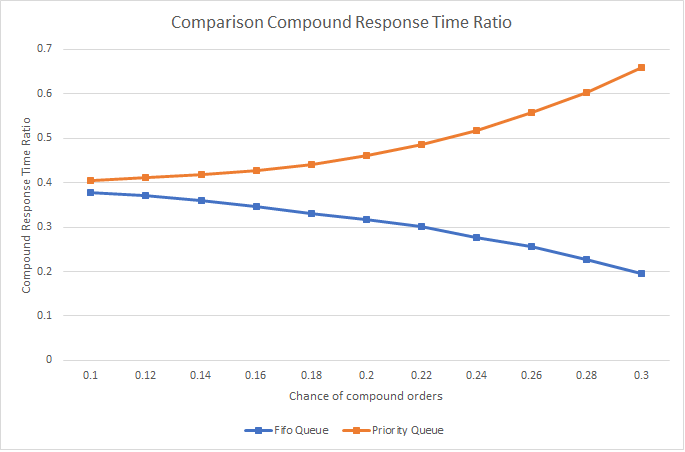
\includegraphics[width=0.75\textwidth]{figs/comparisonQueue.png}
\end{figure}

We can clearly see that by increasing the odds of compound orders, in the fifo case, Vip users tends to lose the "advantage" obtained during the cashier service. So, indeed, by using a priority queue in kitchen we can guarantee an even more privileged service. But is it necessary? Of course not, it depends on the type of service that the Bar Administrator strive to get. In fact we see that even without using a priority queue in the kitchen, the advantage obtained during tha cashier service is enough to let Vip user have some benefits (around 2m) even in case of compound orders:

\begin{figure}[H]
    \centering
    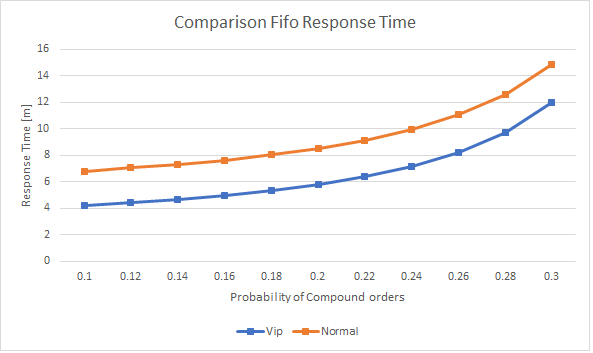
\includegraphics[width=0.75\textwidth]{figs/comparisonFifoKitchen.png}
\end{figure}

\subsection{System Response to different Workloads}

\begin{figure}[H]
    \centering
    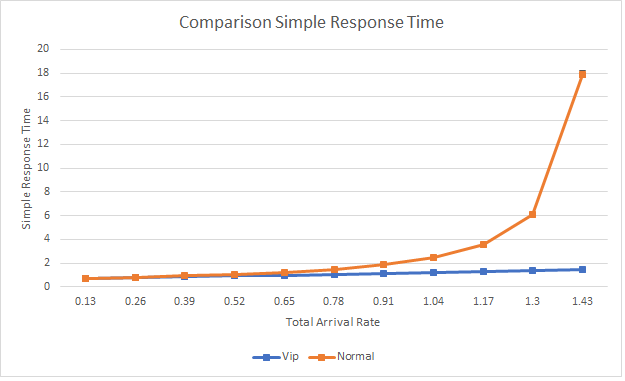
\includegraphics[width=0.75\textwidth]{figs/workloadSimple.png}
\end{figure}

\begin{figure}[H]
    \centering
    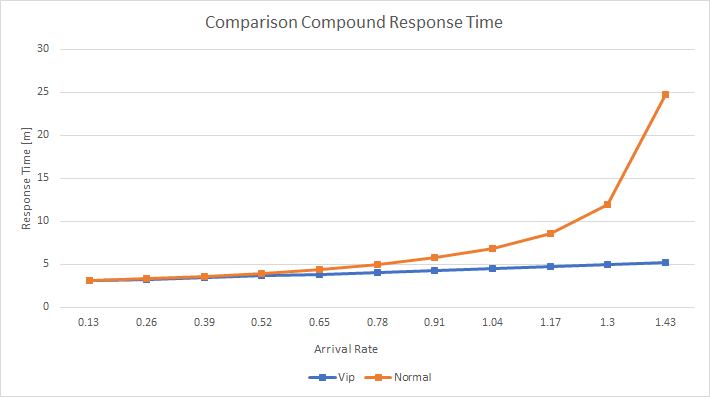
\includegraphics[width=0.75\textwidth]{figs/workloadCompound.png}
\end{figure}

Note that the Inter-Arrival rate for the kitchen with this configuration is actually 0.2 * "value showed in the x axis". We kept those numbers only to let the reader catch the similarities with the previous graph. %TODO da controllare

\subsection{Vip Rate study}

One of the things that should be taken into consideration when fine-tuning the system is the amount of allowed VIP users. Of course if all users are VIP there would be no benefit, all the observation discussed until now would makes no sense and chance are that the few Normal user that comes will never be served. So, in order to decide the correct percentage of allowed VIP users, that permits a reasonable response time for Normal User along with some benefits to the Vip ones, we executed a full factorial analysis with the following configuration:
 
 %TODO configurazione Omnetpp

 By changing only the percentage of VIP users we can set a reasonable response time for Normal user (we opted for 15m) and establish the optimal percentage of Vip users which we found it to be between 10\% and 30\%.

\begin{figure}[H]
    \centering
    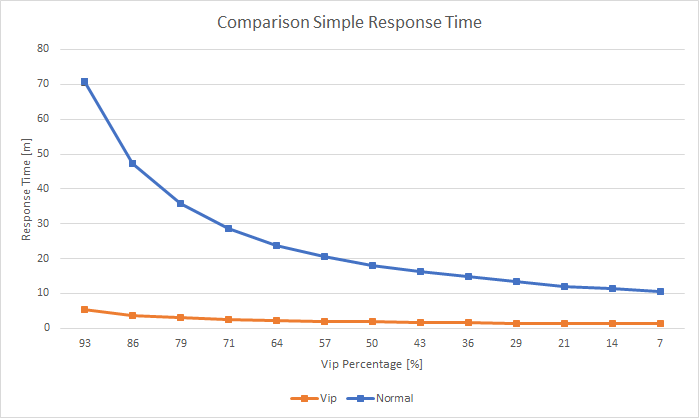
\includegraphics[width=0.75\textwidth]{figs/comparisonSimpleResponseTime.png}
\end{figure}

 We can also plot the simpleResponseTimeRatio with the same configuration and ensure that, in fact, Vip users are at least 80\% faster than Normal users in that range.

\begin{figure}[H]
    \centering
    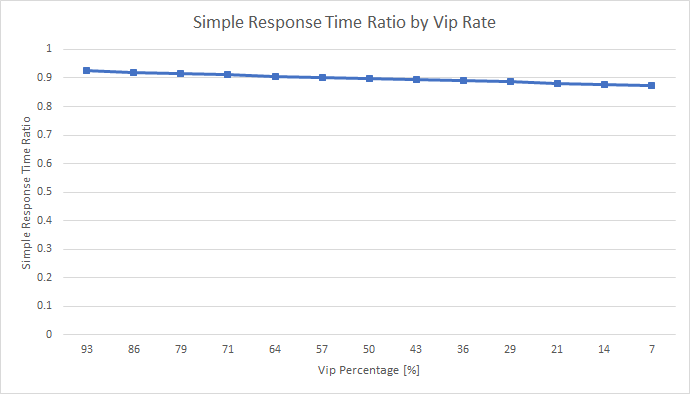
\includegraphics[width=0.75\textwidth]{figs/simpleResponseTimeRatio.png}
\end{figure}


 %Note that we have taken into consideration only the cashier Response Time because there's nothing special going on the kitchen, all users are treated equally. Basically the total Response Time can be seen as %the cashier Response Time plus a constant. %TODO da controllare perche è un'affermazione molto forte


All the above can be repeated for the kitchen in the Priority case to get similar results. In fact we can expect a fairly reasonable response time from normal users in the same range:

\begin{figure}[H]
    \centering
    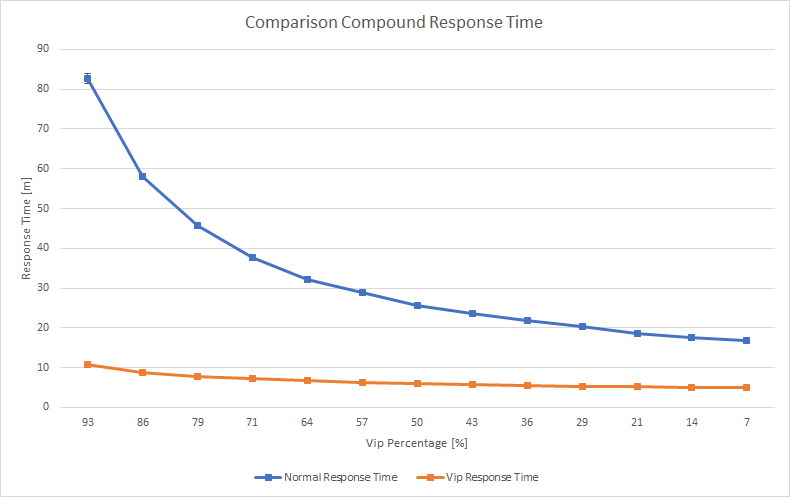
\includegraphics[width=0.75\textwidth]{figs/comparisonCompoundResponseTime.png}
\end{figure}
